\documentclass[submit]{harvardml}

\course{CS181-S20}
\assignment{Assignment \#1}
\duedate{11:59pm February 7, 2020} 

\usepackage[OT1]{fontenc}
\usepackage[colorlinks,citecolor=blue,urlcolor=blue]{hyperref}
\usepackage[pdftex]{graphicx}
\usepackage{graphicx}
\usepackage{caption}
\usepackage{subcaption}
\usepackage{fullpage}
\usepackage{soul}
\usepackage{amsmath}
\usepackage{amssymb}
\usepackage{color}
\usepackage{todonotes}
\usepackage{listings}
\usepackage{common}

\usepackage[mmddyyyy,hhmmss]{datetime}

\definecolor{verbgray}{gray}{0.9}

\lstnewenvironment{csv}{
  \lstset{backgroundcolor=\color{verbgray},
  frame=single,
  framerule=0pt,
  basicstyle=\ttfamily,
  columns=fullflexible}}{}
 

\begin{document}
\begin{center}
{\Large Homework 1: Linear Regression}\\
\end{center}

\subsection*{Introduction}
This homework is on different forms of linear regression and focuses
on loss functions, optimizers, and regularization. Linear regression 
will be one of the few models that we see that has an analytical solution.
These problems focus on deriving these solutions and exploring their 
properties. 

If you find that you are having trouble with the first couple
problems, we recommend going over the fundamentals of linear algebra
and matrix calculus (see links on website).  The relevant parts of the
cs181-textbook notes are Sections 2.1 - 2.7.  We strongly recommend reading the textbook before beginning the homework.

We also encourage you to first read the Bishop
textbook, particularly: Section 2.3 (Properties of Gaussian
Distributions), Section 3.1 (Linear Basis Regression), and Section 3.3
(Bayesian Linear Regression). (Note that our notation is slightly different but
the underlying mathematics remains the same!).

Please type your solutions after the corresponding problems using this
\LaTeX\ template, and start each problem on a new page.

Homeworks will be submitted through Gradescope. You will be added to the course Gradescope once you join the course Canvas page. If you haven?t received an invitation, contact the course staff through Piazza.

Please submit the \textbf{writeup PDF to the Gradescope assignment `HW1'}. Remember to assign pages for each question. 

Please submit your \textbf{\LaTeX file and code files to the Gradescope assignment `HW1 - Supplemental'}. 

You can use a \textbf{maximum of 2 late days} on this assignment.  Late days will be counted based on the latest of the two submissions.
\\

%%%%%%%%%%%%%%%%%%%%%%%%%%%%%%%%%%%%%%%%%%%%%
% Problem 1
%%%%%%%%%%%%%%%%%%%%%%%%%%%%%%%%%%%%%%%%%%%%%

\begin{problem}[Optimizing a Kernel, 15pts]

Kernel-based regression techniques are similar to nearest-neighbor
regressors: rather than fit a parametric model, they predict values
for new data points by interpolating values from existing points in
the training set.  In this problem, we will consider a kernel-based
regressor of the form:
\begin{equation*}
  f(x^*) = \frac{ \sum_{n} K(x_n,x^*) y_n  }{ \sum_{n} K(x_n,x^*) } 
\end{equation*}
where $(x_n,y_n)$ are the training data points, and $K(x,x')$ is a
kernel function that defines the similarity between two inputs $x$ and
$x'$. Assume that each $x_i$ is represented as a row vector, i.e. a
1 by $D$ vector where $D$ is the number of features for each data point. A popular choice of 
kernel is a function that decays as the distance between the two points increases, such as
\begin{equation*}
  K(x,x') = \exp(-||x-x'||^2_2) = \exp(-(x-x') (x-x')^T ) 
\end{equation*} 
However, the squared Euclidean distance $||x-x'||^2_2$ may not always
be the right choice.  In this problem, we will consider optimizing
over squared Mahalanobis distances
\begin{equation*}
  K(x,x') = \exp(-(x-x') W (x-x')^T ) 
  \label{eqn:distance}
\end{equation*} 
where $W$ is a symmetric $D$ by $D$ matrix.  Intuitively, introducing
the weight matrix $W$ allows for different dimensions to matter
differently when defining similarity.

\begin{enumerate}

\item Let $\{(x_n,y_n)\}_{n=1}^N$ be our training data set.  Suppose
  we are interested in minimizing the residual sum of squares.  Write down this
  loss over the training data $\mcL(W)$ as a function of $W$.
  
  Hint:  For each point $(x_i, y_i)$ in the training dataset, consider for which subset of training data you should sum kernel function $K$ over for each $f(x_i)$.

\item In the following, let us assume that $D = 2$.  That means that
  $W$ has three parameters: $W_{11}$, $W_{22}$, and $W_{12} = W_{21}$.
  Expand the formula for the loss function to be a function of these
  three parameters.

\item Consider the following data set:
\begin{csv}
x1 , x2 , y 
  0 , 0 , 0
  0 , .5 , 0
  0 , 1 , 0 
  .5 , 0 , .5
  .5 , .5 , .5
  .5 , 1 , .5
  1 , 0 , 1
  1 , .5 , 1
  1 , 1 , 1 
\end{csv}
And the following kernels:
\begin{equation*} 
W_1 = \alpha \begin{bmatrix}
  1 & 0 \\
  0 & 1 
\end{bmatrix}
\qquad
W_2 = \alpha \begin{bmatrix}
  0.1 & 0 \\
  0 & 1 
\end{bmatrix}
\qquad
W_3 = \alpha \begin{bmatrix}
  1 & 0 \\
  0 & 0.1 
\end{bmatrix}
\end{equation*} 
with $\alpha = 10$. Write some Python code to compute the loss with respect
to each kernel for the dataset provided above. Which kernel does best?  Why?  How does the choice of $\alpha$ affect the loss?  

\item Derive the gradients with respect to each of the parameters in
  $W$.

\item Bonus:  Code up a gradient descent to
  optimize the kernel for the data set above.  Start your gradient
  descent from $W_1$.  Report on what you find.\\
  Gradient descent is discussed in Section 3.4 of the cs181-textbook notes and Section 5.2.4 of Bishop, and will be covered later in the course! 

\end{enumerate}
  
\end{problem}  


\newpage

%%%%%%%%%%%%%%%%%%%%%%%%%%%%%%%%%%%%%%%%%%%%%
% Problem 2
%%%%%%%%%%%%%%%%%%%%%%%%%%%%%%%%%%%%%%%%%%%%%

\begin{problem}[Kernels and kNN, 10pts]

Now, let us compare the kernel-based approach to an approach based on
nearest-neighbors.  Recall that kNN uses a predictor of the form

  \begin{equation*}
    f(x^*) = \frac{1}{k} \sum_n y_n \mathbb{I}(x_n \texttt{ is one of k-closest to } x^*)
  \end{equation*}

 where $\mathbb{I}$ is an indicator variable. For this problem, you will use the same kernels as Problem 1, and dataset \verb|data/p2.csv|.

\begin{enumerate}

\item Make 6 plots using the kernel distance given by $W_1$ from Problem 1.  In each plot,
  you will plot the predicted value of $y$ as the color of each point (grayscale between $0$ and $1$) given $x_1$
  (horizontal axis) and $x_2$ (vertical axis).  For $x_1$ and $x_2$,
  use a grid spaced every 0.1 for $x_1=0$ to $x_1=1$ and $x_2=0$ to
  $x_2=1$.  
  
  For the first three plots, use the kernel-based predictor
  varying $\alpha = \{0.1,3,10\}$.  For the next three plots, use
  the kNN predictor with $\alpha = 1$, $k=\{1,5,15\}$.  Print the least squares loss for each of the 6 plots.
  
  You may choose to use some starter Python code to create your plots provided in \verb|T1_P2.py|.  Please \textbf{write your own implementation of kNN} for full credit.  Do not use external libraries to find nearest neighbors.
  
\item Do any of the kernel-based regression plots look like the 1NN?
  The 15NN?  Why or why not?

\item Do you think that there will always be a version of kernel
  regression (based on varying $\alpha$) that looks like a kNN for any
  $k$, for a fixed distance or kernel function?  Why or why not?
  
\item Why did we not vary $\alpha$ for the kNN approach?    

\end{enumerate}

\end{problem}


\newpage 

%%%%%%%%%%%%%%%%%%%%%%%%%%%%%%%%%%%%%%%%%%%%%
% Problem 3
%%%%%%%%%%%%%%%%%%%%%%%%%%%%%%%%%%%%%%%%%%%%%

\begin{problem}[Deriving Linear Regression, 10pts]

In class, we noted that the solution for the least squares linear regressions ``looked'' like a ratio of covariance and variance terms.  In this problem, we will derive that.  Let us assume the following generative process for our data:

\begin{eqnarray*}
  x &\sim N(0,\Sigma_x) \\
  \epsilon &\sim N(0,\sigma^2)\\
  y | x, \epsilon &= w^Tx + \epsilon 
  \end{eqnarray*}
  
Assume scalar $x$, $\epsilon$, $w$, and $y$, and that $x$ is independent of $\epsilon$.

\begin{enumerate}

\item Provide a formula for $\Sigma_{yx} = E_{x, y}[yx]$ based on the above generative model.

\item Provide a formula to estimate $E_{x, y}[yx]$ given observed data $\{(x_n,y_n)\}_{n=1}^N$.

\item Moment terms like $E_{x, y}[yx]$, $E_{x, y}[xx^T]$, etc. can easily be
  estimated from the data (like you did above).  Write down an
  expression for the optimal $w^*$ which minimizes expected squared residual loss 
  in terms of moments
  (e.g. $\mu_x,\Sigma_x,\Sigma_{yx},\sigma$). Does your expression for optimal $w^*$ match the optimal $w^*$ for least squares linear regression derived in Section 2.6 of the cs181-textbook?

\item Now, suppose the data $x$ were generated from
  $N(\mu_x,\Sigma_x)$.  Write an expression for $w^*$ in terms of
  moments (as above).  
  
\item Would the formula for $w^*$ derived in (3.4) hold if the process generating the $x$'s
  were no longer Gaussian, but still had the same means, variances, and covariances?
  That is, $E[x]=\mu_x$, $Var[x]=\Sigma_x$, $Var[\epsilon] = \sigma^2$, and $E[yx] = \Sigma_{y x}$, but the distribution of $x$
  is not Gaussian?  
  
\end{enumerate}

\end{problem}


%%%%%%%%%%%%%%%%%%%%%%%%%%%%%%%%%%%%%%%%%%%%%
% Problem 4
%%%%%%%%%%%%%%%%%%%%%%%%%%%%%%%%%%%%%%%%%%%%%

\begin{problem}[Modeling Changes in Republicans and Sunspots, 15pts]
  
 The objective of this problem is to learn about linear regression
 with basis functions by modeling the number of Republicans in the
 Senate. The file \verb|data/year-sunspots-republicans.csv| contains the
 data you will use for this problem.  It has three columns.  The first
 one is an integer that indicates the year.  The second is the number
 of Sunspots observed in that year.  The third is the number of Republicans in the Senate for that year.
 The data file looks like this:
 \begin{csv}
Year,Sunspot_Count,Republican_Count
1960,112.3,36
1962,37.6,34
1964,10.2,32
1966,47.0,36
\end{csv}

You can see scatterplots of the data in the figures below.  The horizontal axis is the Year, and the vertical axis is the Number of Republicans and the Number of Sunspots, respectively.

\begin{center}
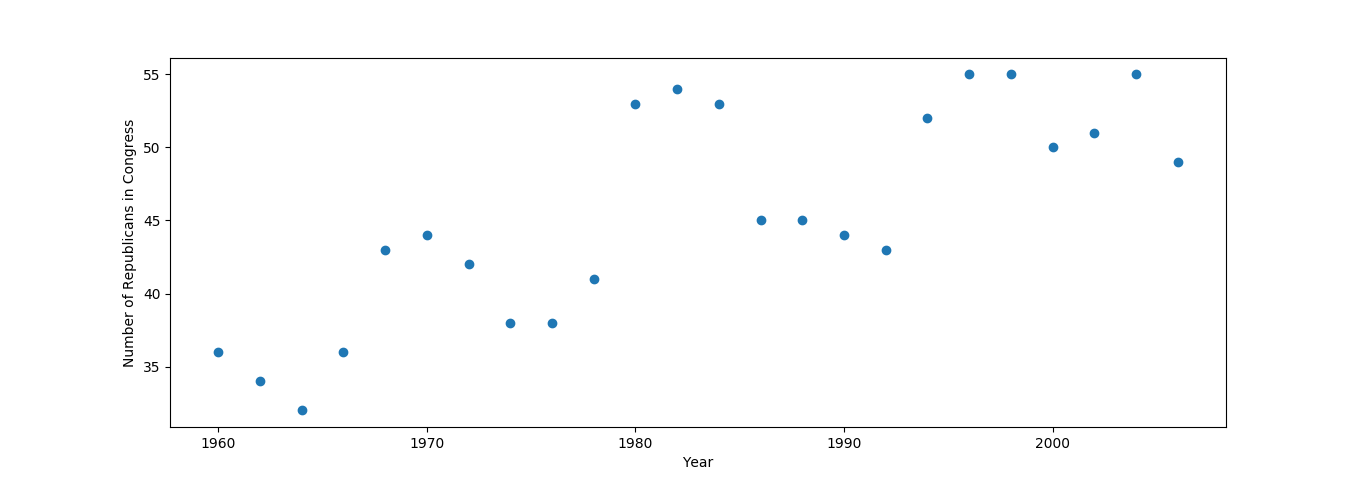
\includegraphics[width=.5\textwidth]{data/year-republicans}
\end{center}

\begin{center}
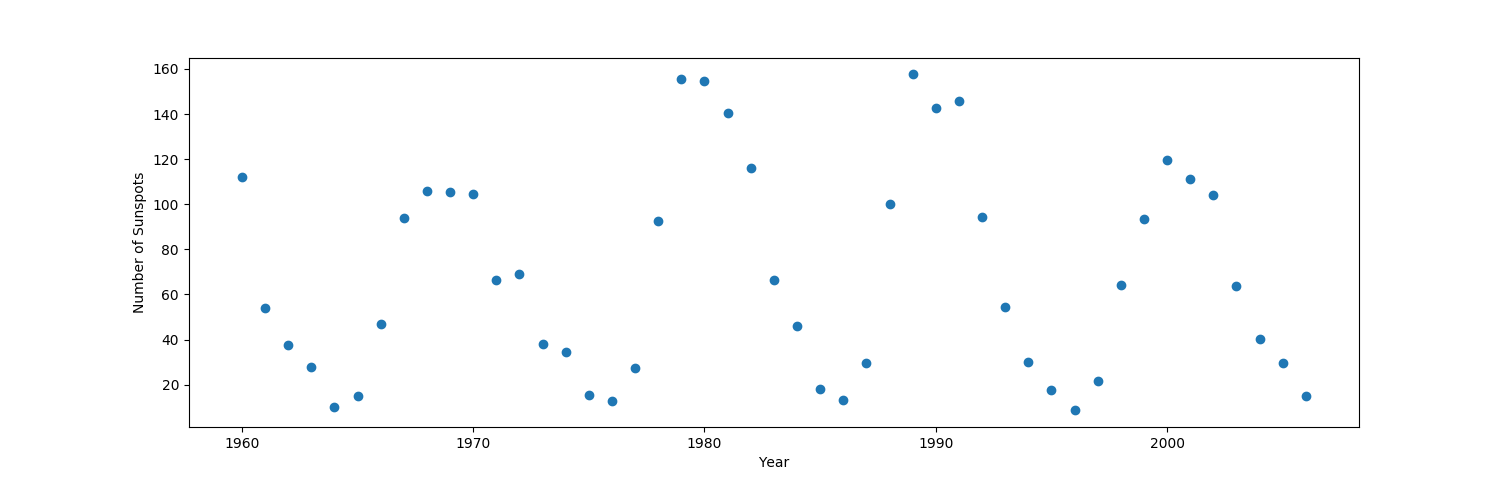
\includegraphics[width=.5\textwidth]{data/year-sunspots}
\end{center}

(Data Source: \url{http://www.realclimate.org/data/senators_sunspots.txt})\\
\vspace{-5mm}

\begin{enumerate}

\item In this problem you will implement ordinary least squares regression using 4 different basis functions for
\textbf{Year (x-axis)} v. \textbf{Number of Republicans in the Senate (y-axis)}. Some starter Python code
that implements simple linear regression is provided in \verb|T1_P3.py|.

First, plot the data and regression lines for each of the following sets of basis functions, and include
the generated plot as an image in your submission PDF. You will therefore make 4 total plots:
\begin{enumerate}
	\item[(a)] $\phi_j(x) = x^j$ for $j=1, \ldots, 5$\\
    ie, use basis $y = a_1 x^1 + a_2 x^2 + a_3 x^3 + a_4 x^4 + a_5 x^5$ for some constants $\{a_1, ..., a_5\}$. 
    \item[(b)] $\phi_j(x) = \exp{\frac{-(x-\mu_j)^2}{25}}$ for $\mu_j=1960, 1965, 1970, 1975, \ldots 2010$
	\item[(c)] $\phi_j(x) = \cos(x / j)$ for $j=1, \ldots, 5$
	\item[(d)] $\phi_j(x) = \cos(x / j)$ for $j=1, \ldots, 25$
\end{enumerate}
\vspace{-2mm}
{\footnotesize * Note: Be sure to add a bias term for each of the basis functions above.}

Second, for each plot include the residual sum of squares error.

\item Repeat the same exact process as above but for \textbf{Number of Sunspots (x-axis)} v. \textbf{Number of Republicans in the Senate (y-axis)}. Now, however, only use data from before 1985, and only use basis functions (a), (c), and (d) -- ignore basis (b). You will therefore make 3 total plots. For each plot make sure to also include the residual sum of squares error.

Which of the three bases (a, c, d) provided the "best" fit? \textbf{Choose one}, and keep in mind the generalizability of the model. 

Given the quality of this fit, do you believe that the number of sunspots controls the number of Republicans in the senate (Yes or No)?

\end{enumerate}

\end{problem}



\newpage
%%%%%%%%%%%%%%%%%%%%%%%%%%%%%%%%%%%%%%%%%%%%%
% Name and Calibration
%%%%%%%%%%%%%%%%%%%%%%%%%%%%%%%%%%%%%%%%%%%%%
\subsection*{Name}

\subsection*{Collaborators and Resources}
Whom did you work with, and did you use any resources beyond cs181-textbook and your notes?

\subsection*{Calibration}
Approximately how long did this homework take you to complete (in hours)? 

\end{document}


